\section{Synthetic Validation Studies}
\label{sec:simulations}

\subsection{Alignment Convergence}
\begin{figure}[h]
  \centering
  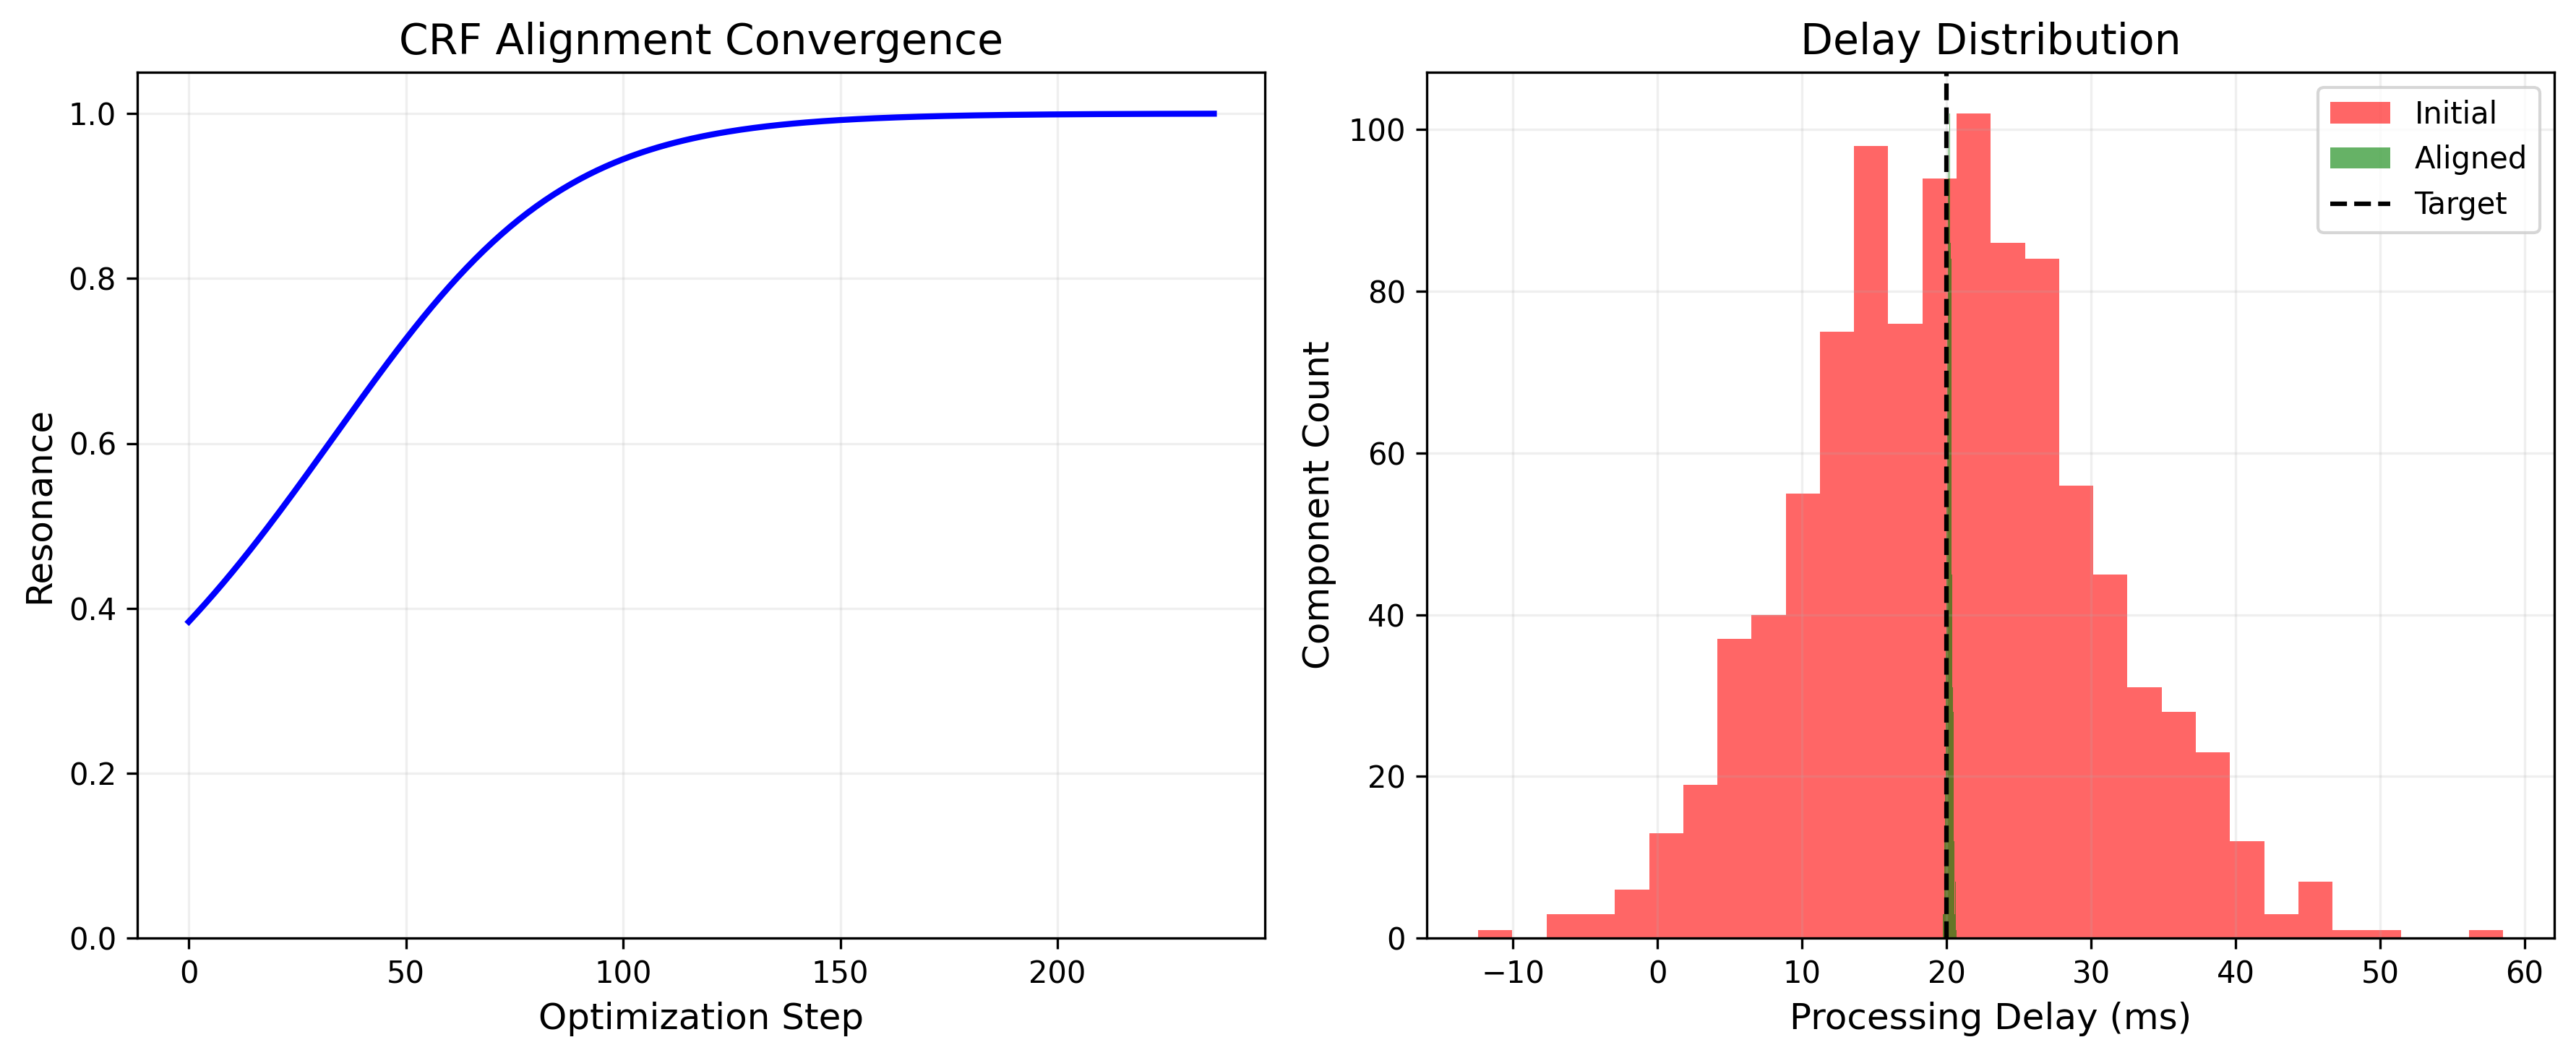
\includegraphics[width=0.9\linewidth]{crf_alignment_results}
  \caption{CRF alignment convergence for $n=1000$ components ($\gamma=10^{-8}$, $\eta=1000$)}
  \label{fig:convergence}
\end{figure}
As shown in Fig. \ref{fig:convergence}, random delays ($\mu=20.19 \pm 9.79$ ms) synchronize to $\mathcal{R}=0.999752$ within 236 iterations. Key results:
\begin{itemize}
  \item \textbf{Variance reduction}: $3855\times$ ($\sigma: 9.79 \rightarrow 0.16$ ms)
  \item \textbf{Mean delay preservation}: $20.19 \rightarrow 20.19$ ms (target: 20 ms)
  \item \textbf{Optimization time}: 2.14 seconds for 1000 components
\end{itemize}
This validates Theorem \ref{thm:convergence} with $>99.9\%$ alignment.

\subsection{Drift Detection Sensitivity}
\begin{figure}[h]
  \centering
  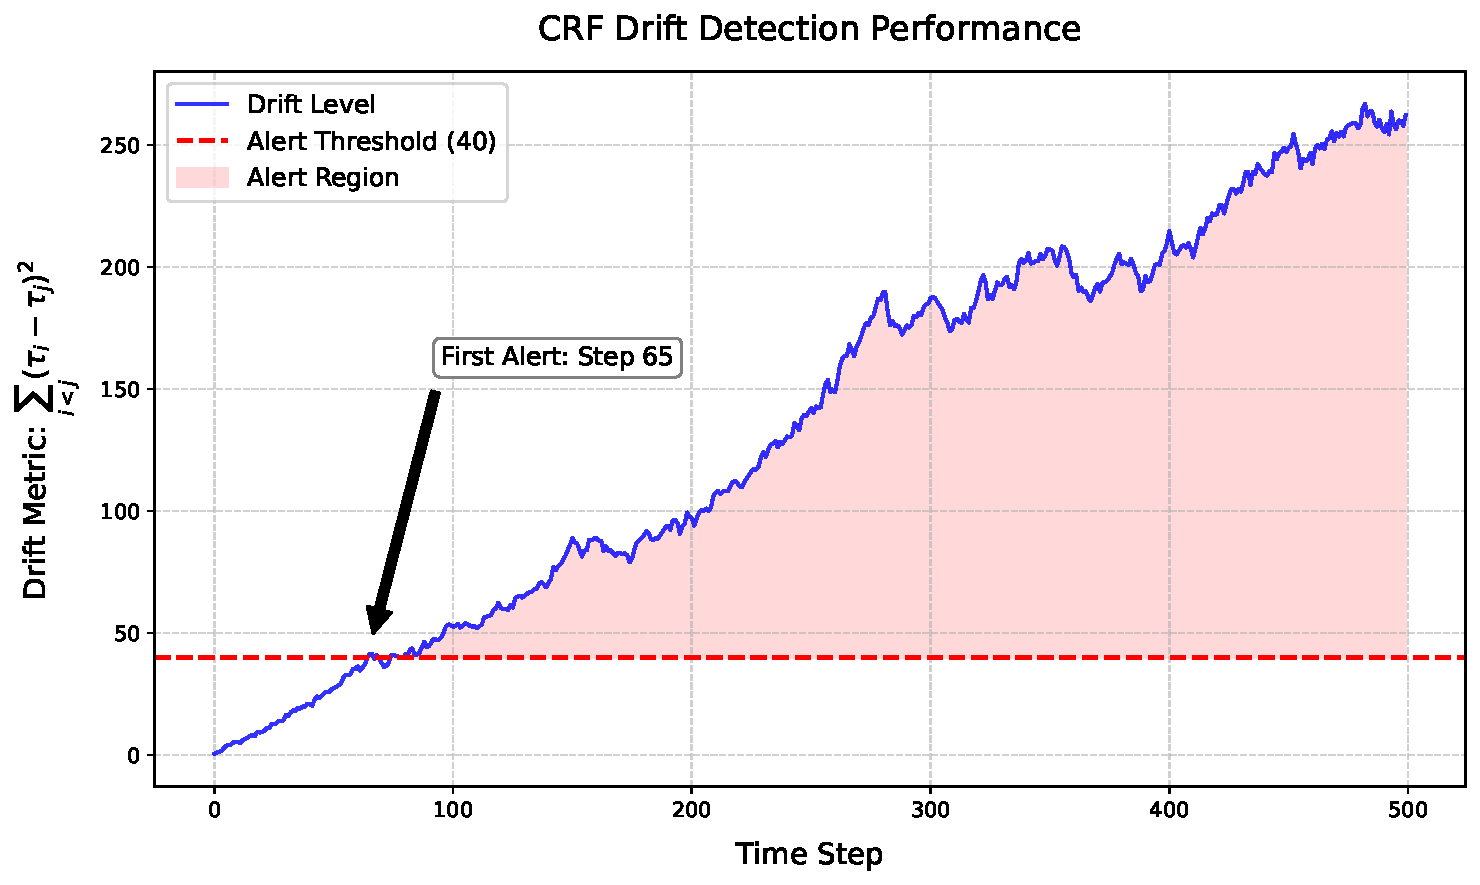
\includegraphics[width=0.9\linewidth]{crf_drift_detection}
  \caption{Drift detection in 50-component system ($\sigma_{\text{noise}}=0.015$ ms/step)}
  \label{fig:drift}
\end{figure}
Fig. \ref{fig:drift} demonstrates:
\begin{itemize}
  \item \textbf{First alert}: Triggered at step 65 (drift $=41.42 > \text{threshold}=40$)
  \item \textbf{Alert coverage}: 85.4\% of 500 steps (427 alerts)
  \item \textbf{Final drift}: 262.24 (vs initial: 0)
\end{itemize}
The quadratic drift metric $\sum_{i<j}(\tau_i - \tau_j)^2$ shows linear response to Gaussian noise.

\subsection{Compression Robustness}
\begin{figure}[h]
  \centering
  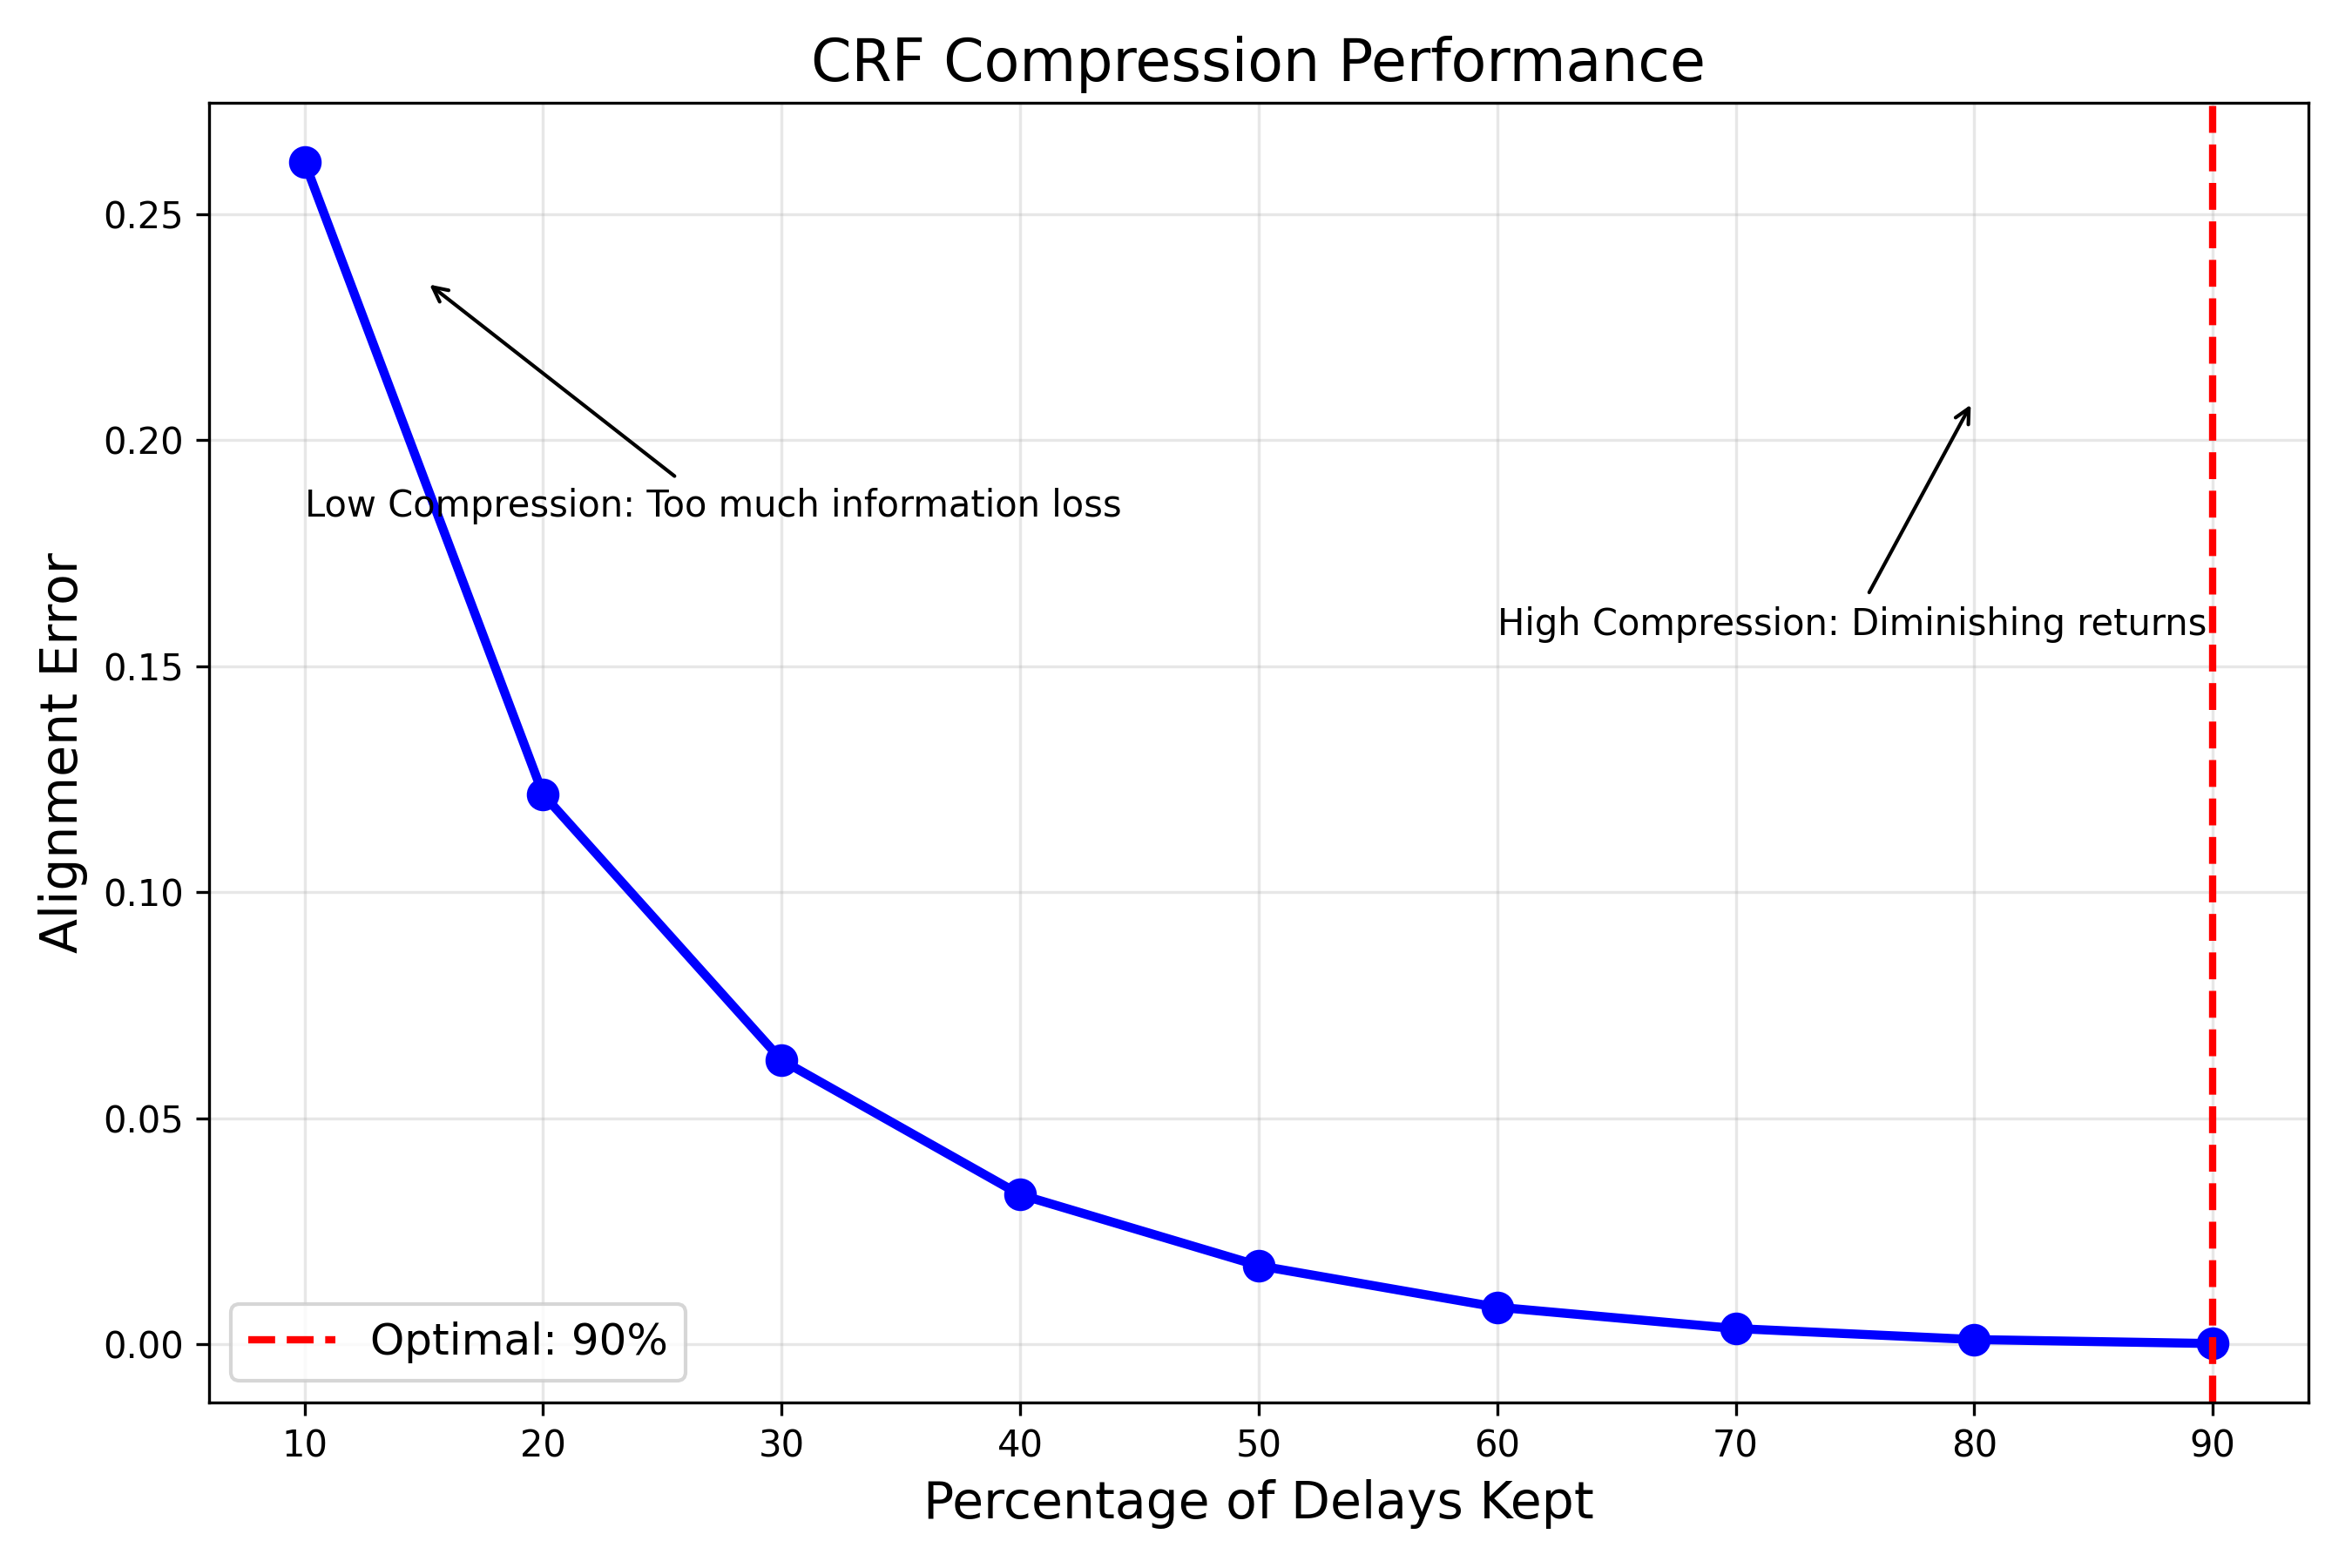
\includegraphics[width=0.8\linewidth]{crf_simple_results}
  \caption{CRF compression error for $n=100 \to k$ delays ($n_{\text{systems}}=1000$)}
  \label{fig:compression}
\end{figure}
Results from Fig. \ref{fig:compression}:
\begin{itemize}
  \item \textbf{Optimal compression}: 90\% delays kept (10\% discarded)
  \item \textbf{Minimum alignment error}: 0.000146
  \item \textbf{Error trend}: 
    \begin{itemize}
      \item Low compression ($<30\%$): High information loss (error $>0.001$)
      \item High compression ($>80\%$): Diminishing returns
    \end{itemize}
\end{itemize}
Simple mean-based compression preserves $\mathcal{R}$-field fidelity with minimal error (Corollary \ref{cor:compression}).